\documentclass[../main.tex]{subfiles}

\begin{titlepage}

%\sffamily

\raggedleft

\vspace*{-2cm}

%
\includegraphics{logo-th-rosenheim-2019_master_quer_2c}

\vfill

\centering
\LARGE
% \vspace*{\fill}
%-----------
Fakultät Maschinenbau und Mechatronik  \vspace{0.5cm}\\
\Large
Studiengang Maschinenbau

\vspace{2cm}

\LARGE

Kinematische Simulation des Wälzfräsens im Überlagerungsverfahren

\vspace{2cm}

\Large
Bachelor Thesis

\vspace{1.5cm}


\Large
von

\vspace{0.5cm}

%\vspace*{\fill}

\LARGE
Christopher Schuster \vspace{1cm}

\vspace{1cm}

\flushleft
 \Large
\vspace*{\fill}

\begin{tabbing}
Datum der Abgabe: \= tt.mm.jjjj \kill
Datum der Abgabe: \> \today \\
Erstprüfer: \> Prof.\ Dr.-Ing.\ Stefan Scherbarth \\
Zweitprüfer: \> Prof.\ Dr.\
\end{tabbing}

\end{titlepage}

% einbinden der erklärungsseite
\begin{tikzpicture}[remember picture,overlay]
	\node at (current page.center) {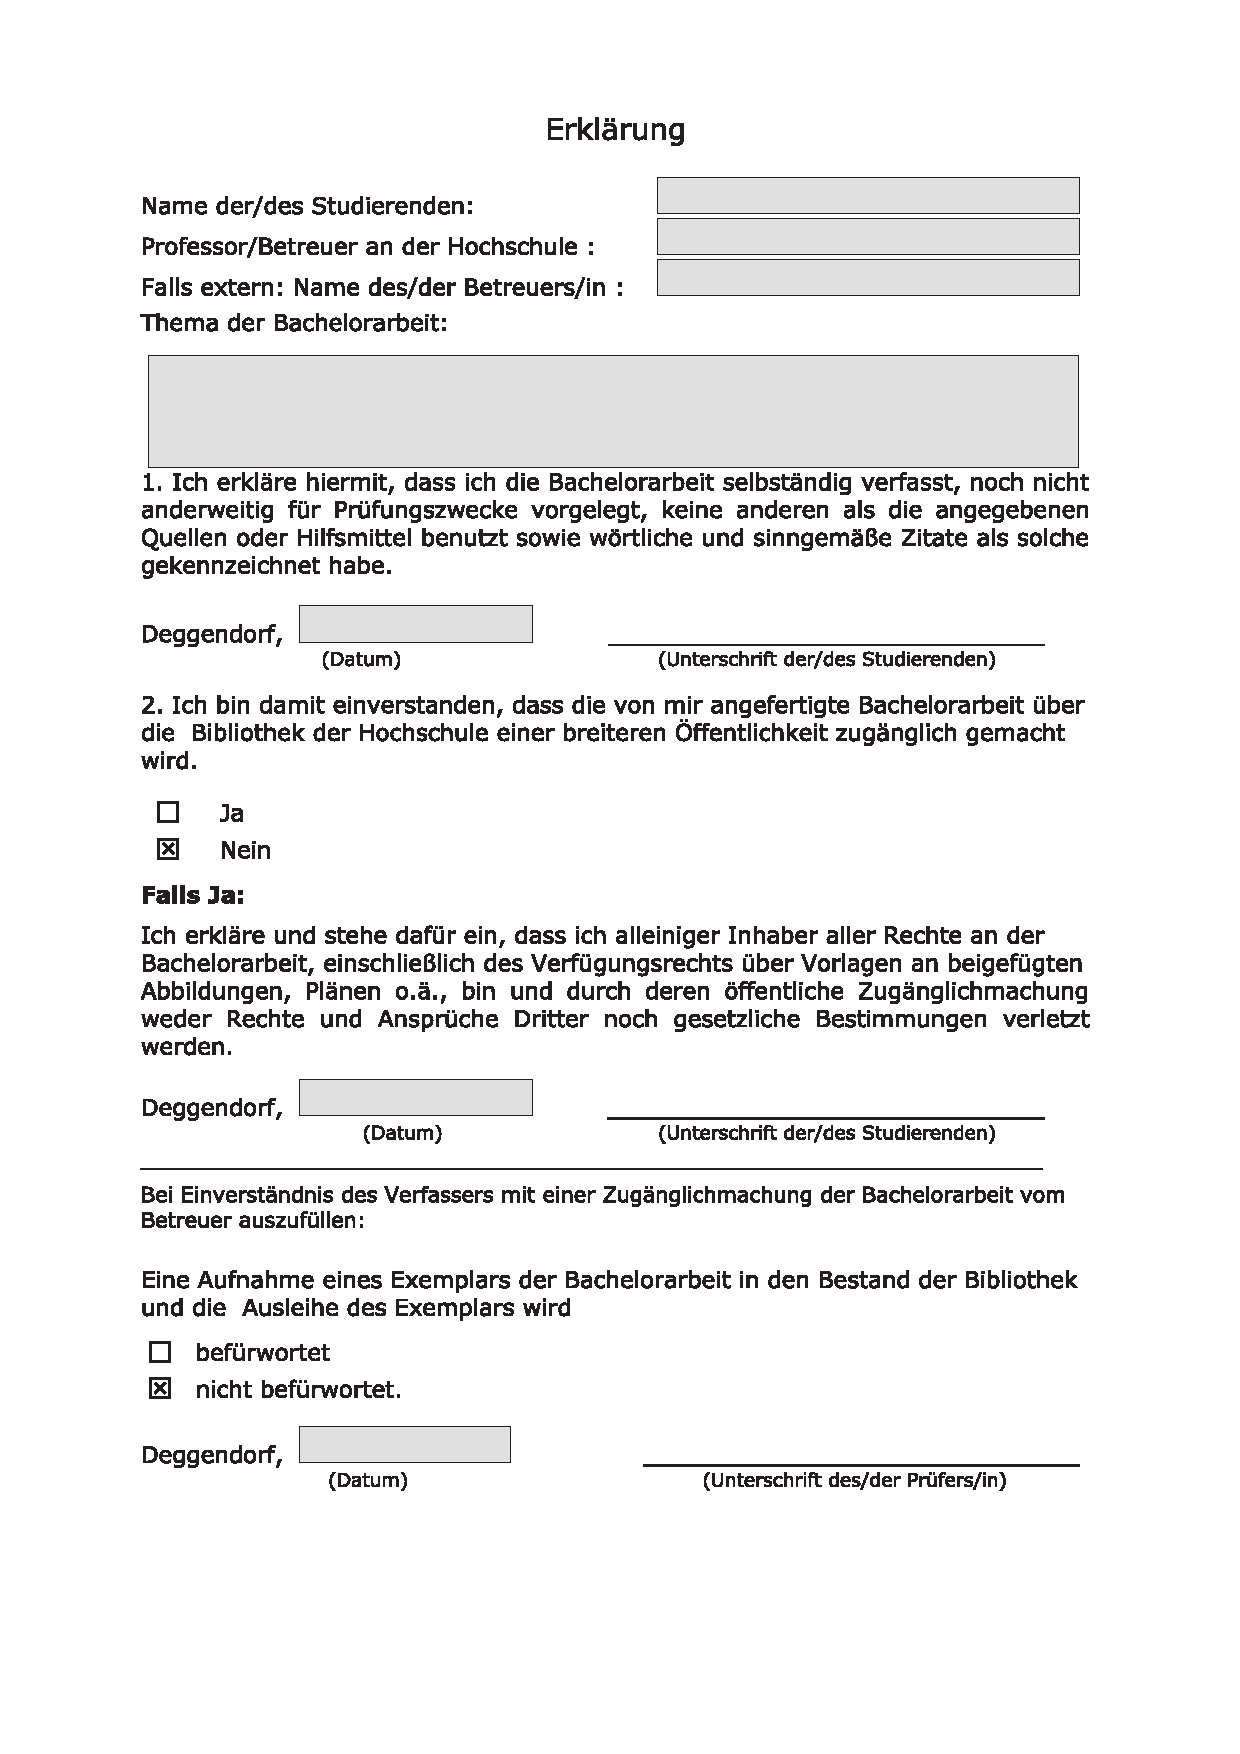
\includegraphics{erklaerung}};
	\begin{scope}[shift={(current page.south west)},every node/.style={anchor=base west}]
		\node at (5.5cm,18.975cm) {\sffamily\today};
	\end{scope}
\end{tikzpicture}


%%% Local Variables: 
%%% mode: latex
%%% TeX-master: "d"
%%% End: 
